% Template for a Computer Science Tripos Part II project dissertation
\documentclass[12pt,a4paper,twoside,openright]{report}
\usepackage[pdfborder={0 0 0}]{hyperref}    % turns references into hyperlinks
\usepackage[margin=25mm]{geometry}  % adjusts page layout
\usepackage{graphicx}  % allows inclusion of PDF, PNG and JPG images
\usepackage{verbatim}
\usepackage{docmute}   % only needed to allow inclusion of proposal.tex
\usepackage[utf8]{inputenc}
\usepackage{mathtools}
\usepackage{changepage}
\usepackage{url}
\usepackage{blindtext}

%\raggedbottom                           % try to avoid widows and orphans
\sloppy
\clubpenalty1000%
\widowpenalty1000%

\renewcommand{\baselinestretch}{1.1}    % adjust line spacing to make
                                        % more readable

\begin{document}

% Change these

\newcommand{\mcandidate}{2416B}
\newcommand{\mfullname}{Jude Howard-Gluckstein Tyrrell}
\newcommand{\mcollege}{Homerton College}
\newcommand{\mtitle}{Notation for Phonological Audio Composition}
\newcommand{\mexamination}{Computer Science Tripos -- Part II}
\newcommand{\mdate}{May 2023}
\newcommand{\moriginator}{Prof. Alan Blackwell}
\newcommand{\msupervisor}{Prof. Alan Blackwell}
\newcommand{\mwordcount}{10814}
\newcommand{\mlinecount}{0}
% Consent to the dissertation made available to University members
\newcommand{\mconsent}{I am content for my dissertation to be made available to the students and staff of the University.}
% For the Declaration of originality
\newcommand{\msignature}{Jude Tyrrell}


\bibliographystyle{plain}


%%%%%%%%%%%%%%%%%%%%%%%%%%%%%%%%%%%%%%%%%%%%%%%%%%%%%%%%%%%%%%%%%%%%%%%%
% Title


\thispagestyle{empty}

\rightline{\LARGE \textbf{\mfullname}}

\vspace*{60mm}
\begin{center}
\Huge
\textbf{\mtitle} \\[5mm]
\mexamination \\[5mm]
\mcollege \\[5mm]
\mdate  % today's date
\end{center}

%%%%%%%%%%%%%%%%%%%%%%%%%%%%%%%%%%%%%%%%%%%%%%%%%%%%%%%%%%%%%%%%%%%%%%%%%%%%%%
% Proforma, table of contents and list of figures

\pagestyle{plain}

\newpage
\newpage
\section*{Declaration of originality}

I, \mfullname{} of \mcollege, being a candidate for Part II of the Computer Science Tripos, hereby declare that this dissertation and the work described in it are my own work, unaided except as may be specified below, and that the dissertation does not contain material that has already been used to any substantial extent for a comparable purpose. \mconsent

\bigskip
\leftline{Signed \msignature}
\bigskip
\leftline{Date \today}

\chapter*{Proforma}

{\large
\begin{tabular}{ll}
Candidate Number:   & \bf \mcandidate                   \\
Project Title:      & \bf \mtitle                       \\
Examination:        & \bf \mexamination, \mdate         \\
Word Count:         & \bf \mwordcount\footnotemark[1]   \\
Code Line Count:    & \bf \mlinecount                   \\
Project Originator: & \bf \moriginator                  \\
Supervisor:         & \bf \msupervisor                  \\ 
\end{tabular}
}
\footnotetext[1]{This word count was computed
by \texttt{detex diss.tex | tr -cd '0-9A-Za-z $\tt\backslash$n' | wc -w}
}
\stepcounter{footnote}


\section*{Original Aims of the Project}
% At most 100 words

To write a demonstration dissertation\footnote{A normal footnote without the
complication of being in a table.} using \LaTeX\ to save
student's time when writing their own dissertations. The dissertation
should illustrate how to use the more common \LaTeX\ constructs. It
should include pictures and diagrams to show how these can be
incorporated into the dissertation.  It should contain the entire
\LaTeX\ source of the dissertation and the makefile.  It should
explain how to construct an MSDOS disk of the dissertation in
Postscript format that can be used by the book shop for printing, and,
finally, it should have the prescribed layout and format of a diploma
dissertation.


\section*{Work Completed}
% At most 100 words

All that has been completed appears in this dissertation.

\section*{Special Difficulties}
% At most 100 words

Learning how to incorporate encapulated postscript into a \LaTeX\
document on both Ubuntu Linux and OS X.

\newpage

\tableofcontents

\listoffigures

\newpage
\section*{Acknowledgements}

This document owes much to an earlier version written by Simon Moore
\cite{Moore95}.  His help, encouragement and advice was greatly 
appreciated.

%%%%%%%%%%%%%%%%%%%%%%%%%%%%%%%%%%%%%%%%%%%%%%%%%%%%%%%%%%%%%%%%%%%%%%%
% now for the chapters

\pagestyle{headings}

\chapter{Introduction}

\section{Overview of the files}

This document consists of the following files:

\begin{itemize}
\item \texttt{makefile} --- The makefile for the dissertation and
                         Project Proposal
\item \texttt{main.tex} --- The dissertation
\item \texttt{proposal.tex}  --- The project proposal 
\item \texttt{figs} -- A directory containing diagrams and pictures
\item \texttt{refs.bib} --- The bibliography database
\end{itemize}

\section{Building the document}

This document was produced using \LaTeXe which is based upon
\LaTeX\cite{Lamport86}.  To build the document you first need to
generate \texttt{diss.aux} which, amongst other things, contains the
references used.  This if done by executing the command:

\texttt{pdflatex main}

\noindent
Then the bibliography can be generated from \texttt{refs.bib} using:

\texttt{bibtex main}

\noindent
Finally, to ensure all the page numbering is correct run \texttt{pdflatex}
on \texttt{diss.tex} until the \texttt{.aux} files do not change.  This
usually takes 2 more runs.

\subsection{The makefile}

To simplify the calls to \texttt{pdflatex} and \texttt{bibtex}, 
a makefile has been provided, see Appendix~\ref{makefile}. 
It provides the following facilities:

\begin{description}

\item\texttt{make} \\
 Display help information.

\item\texttt{make proposal.pdf} \\
 Format the proposal document as a PDF.

\item\texttt{make view-proposal} \\
 Run \texttt{make proposal.pdf} and then display it with a Linux PDF viewer
 (preferably ``okular'', if that is not available fall back to ``evince'').

\item\texttt{make main.pdf} \\
 Format the dissertation document as a PDF.

\item\texttt{make count} \\
Display an estimate of the word count.

\item\texttt{make all} \\
Construct \texttt{proposal.pdf} and \texttt{diss.pdf}.

\item\texttt{make pub} \\ Make \texttt{diss.pdf}
and place it in my \texttt{public\_html} directory.

\item\texttt{make clean} \\ Delete all intermediate files except the
source files and the resulting PDFs. All these deleted files can
be reconstructed by typing \texttt{make all}.

\end{description}


\section{Counting words}

An approximate word count of the body of the dissertation may be
obtained using:

\texttt{wc main.tex}

\noindent
Alternatively, try something like:

\verb/detex main.tex | tr -cd '0-9A-Z a-z\n' | wc -w/


\chapter{Preparation}

This chapter is empty!


\chapter{Implementation}

\section{Verbatim text}

Verbatim text can be included using \verb|\begin{verbatim}| and
\verb|\end{verbatim}|. I normally use a slightly smaller font and
often squeeze the lines a little closer together, as in:

{\renewcommand{\baselinestretch}{0.8}\small
\begin{verbatim}
GET "libhdr"
 
GLOBAL { count:200; all  }
 
LET try(ld, row, rd) BE TEST row=all
                        THEN count := count + 1
                        ELSE { LET poss = all & ~(ld | row | rd)
                               UNTIL poss=0 DO
                               { LET p = poss & -poss
                                 poss := poss - p
                                 try(ld+p << 1, row+p, rd+p >> 1)
                               }
                             }
LET start() = VALOF
{ all := 1
  FOR i = 1 TO 12 DO
  { count := 0
    try(0, 0, 0)
    writef("Number of solutions to %i2-queens is %i5*n", i, count)
    all := 2*all + 1
  }
  RESULTIS 0
}
\end{verbatim}
}

\section{Tables}

\begin{samepage}
Here is a simple example\footnote{A footnote} of a table.

\begin{center}
\begin{tabular}{l|c|r}
Left      & Centred & Right \\
Justified &         & Justified \\[3mm]
%\hline\\%[-2mm]
First     & A       & XXX \\
Second    & AA      & XX  \\
Last      & AAA     & X   \\
\end{tabular}
\end{center}

\noindent
There is another example table in the proforma.
\end{samepage}

\section{Simple diagrams}

Simple diagrams can be written directly in \LaTeX.  For example, see
figure~\ref{latexpic1} on page~\pageref{latexpic1} and see
figure~\ref{latexpic2} on page~\pageref{latexpic2}.

\begin{figure}
\setlength{\unitlength}{1mm}
\begin{center}
\begin{picture}(125,100)
\put(0,80){\framebox(50,10){AAA}}
\put(0,60){\framebox(50,10){BBB}}
\put(0,40){\framebox(50,10){CCC}}
\put(0,20){\framebox(50,10){DDD}}
\put(0,00){\framebox(50,10){EEE}}

\put(75,80){\framebox(50,10){XXX}}
\put(75,60){\framebox(50,10){YYY}}
\put(75,40){\framebox(50,10){ZZZ}}

\put(25,80){\vector(0,-1){10}}
\put(25,60){\vector(0,-1){10}}
\put(25,50){\vector(0,1){10}}
\put(25,40){\vector(0,-1){10}}
\put(25,20){\vector(0,-1){10}}

\put(100,80){\vector(0,-1){10}}
\put(100,70){\vector(0,1){10}}
\put(100,60){\vector(0,-1){10}}
\put(100,50){\vector(0,1){10}}

\put(50,65){\vector(1,0){25}}
\put(75,65){\vector(-1,0){25}}
\end{picture}
\end{center}
\caption{A picture composed of boxes and vectors.}
\label{latexpic1}
\end{figure}

\begin{figure}
\setlength{\unitlength}{1mm}
\begin{center}

\begin{picture}(100,70)
\put(47,65){\circle{10}}
\put(45,64){abc}

\put(37,45){\circle{10}}
\put(37,51){\line(1,1){7}}
\put(35,44){def}

\put(57,25){\circle{10}}
\put(57,31){\line(-1,3){9}}
\put(57,31){\line(-3,2){15}}
\put(55,24){ghi}

\put(32,0){\framebox(10,10){A}}
\put(52,0){\framebox(10,10){B}}
\put(37,12){\line(0,1){26}}
\put(37,12){\line(2,1){15}}
\put(57,12){\line(0,2){6}}
\end{picture}

\end{center}
\caption{A diagram composed of circles, lines and boxes.}
\label{latexpic2}
\end{figure}



\section{Adding more complicated graphics}

The use of \LaTeX\ format can be tedious and it is often better to use
encapsulated postscript (EPS) or PDF to represent complicated graphics.
Figure~\ref{epsfig} and~\ref{xfig} on page \pageref{xfig} are
examples. The second figure was drawn using \texttt{xfig} and exported in
{\tt.eps} format. This is my recommended way of drawing all diagrams.


\begin{figure}[tbh]
\centerline{
\includegraphics{figs/cuarms.pdf}}
\caption{Example figure using encapsulated postscript}
\label{epsfig}
\end{figure}

\begin{figure}[tbh]
\vspace{4in}
\caption{Example figure where a picture can be pasted in}
\label{pastedfig}
\end{figure}


\begin{figure}[tbh]
\centerline{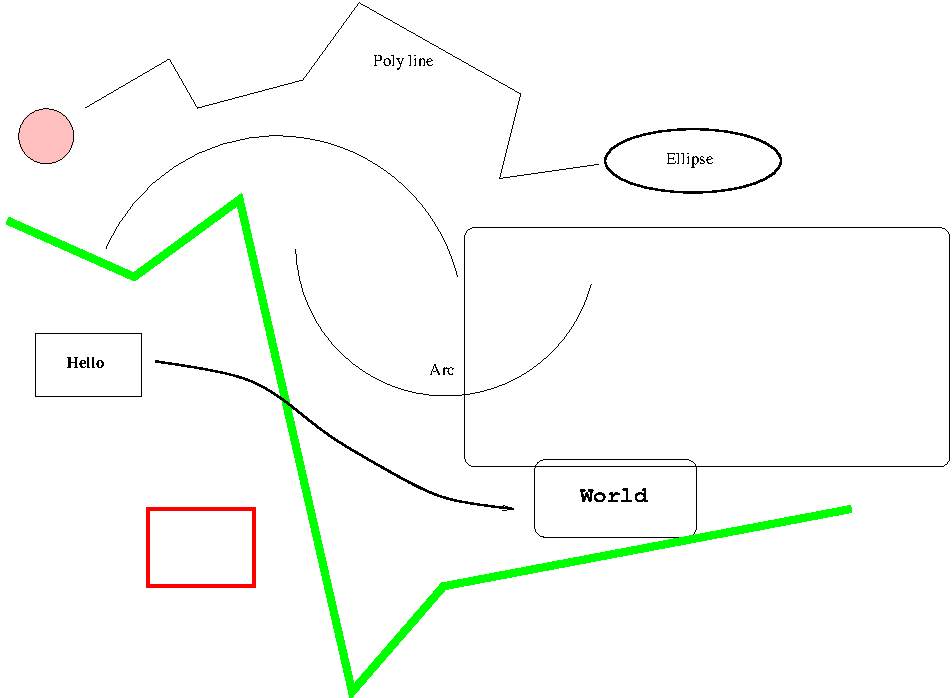
\includegraphics{figs/diagram.pdf}}
\caption{Example diagram drawn using \texttt{xfig}}
\label{xfig}
\end{figure}


\chapter{Evaluation}

\section{Printing and binding}

Use a ``duplex'' laser printer that can print on both sides to print
two copies of your dissertation. Then bind them, for example using the
comb binder in the Computer Laboratory Library.

\section{Further information}

See the Unix Tools notes at

\url{http://www.cl.cam.ac.uk/teaching/current-1/UnixTools/materials.html}


\chapter{Conclusions}

I hope that this rough guide to writing a dissertation is \LaTeX\ has
been helpful and saved you time.


%%%%%%%%%%%%%%%%%%%%%%%%%%%%%%%%%%%%%%%%%%%%%%%%%%%%%%%%%%%%%%%%%%%%%
% the bibliography
\addcontentsline{toc}{chapter}{Bibliography}
\bibliography{refs}

%%%%%%%%%%%%%%%%%%%%%%%%%%%%%%%%%%%%%%%%%%%%%%%%%%%%%%%%%%%%%%%%%%%%%
% the appendices
\appendix

\chapter{Latex source}

\section{metadata.tex}
{\scriptsize\verbatiminput{metadata.tex}}

\section{main.tex}
{\scriptsize\verbatiminput{main.tex}}

\section{proposal.tex}
{\scriptsize\verbatiminput{proposal.tex}}

\chapter{Makefile}

\section{makefile}\label{makefile}
{\scriptsize\verbatiminput{makefile.txt}}

\section{refs.bib}
{\scriptsize\verbatiminput{refs.bib}}


\chapter{Project Proposal}

\documentclass{article}
\usepackage[utf8]{inputenc}
\usepackage{graphicx}
\usepackage[indent=0pt,skip=10pt]{parskip}
\usepackage[a4paper, total={6in,8in}]{geometry}

\begin{document}

\section*{Introduction}

There exists a wide variety of digital tools to aid the composition of music. Modern DAWs (Digital Audio Workstations) such as Ableton and Fruity Loops are used extensively in the recording, mixing and mastering of most of the music that is produced today. These applications are designed to allow musicians to easily rearrange, layer and manipulate snippets of audio which can be imported from external sources, recorded onto the tracks or generated by MIDI instruments. While this design makes musical composition and recording simple and accessible for many popular styles of music, it can be restricting to other styles of composition and inhibit explorations into more niche musical expressions. 
\begin{figure}[h]
    \centering
    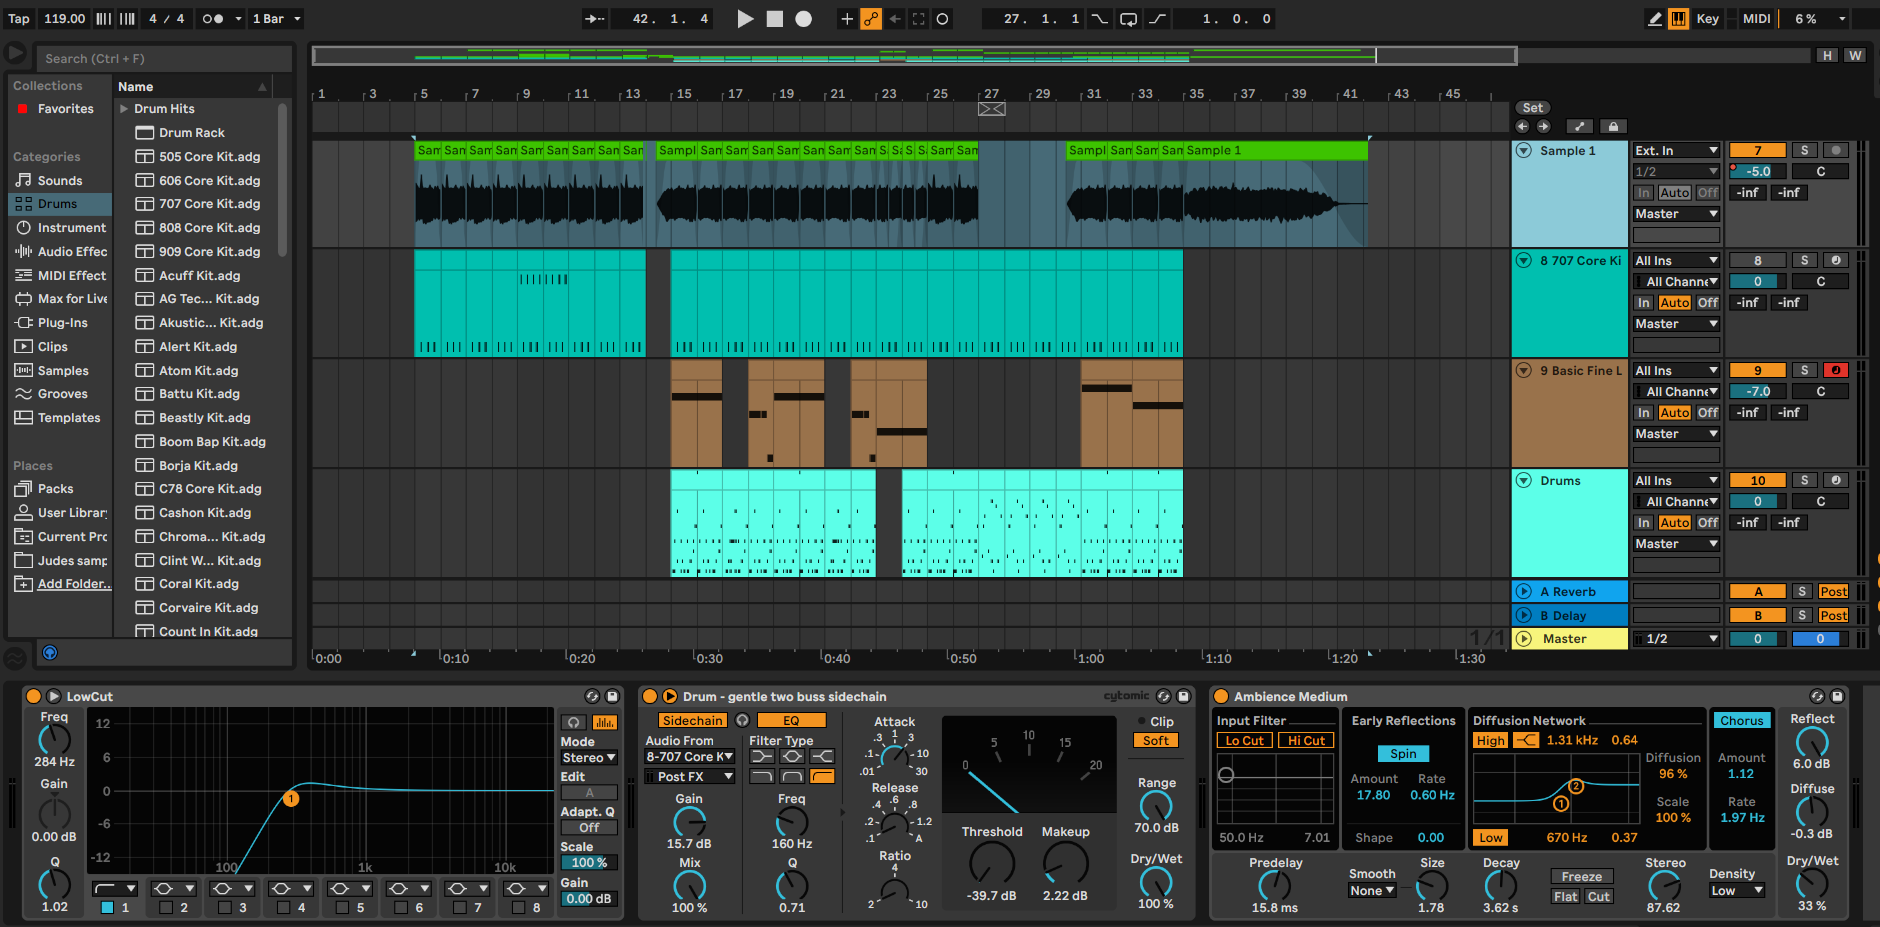
\includegraphics[scale=0.3]{images/ableton example.png}
    \caption{An example of an industry-standard DAW (Ableton 11)}
    \label{fig:ableton}
\end{figure}

Another style of digital music composition that is particularly relevant to my project is through live coding techniques. Live coding (with regards to musical composition) is a performance art in which the artist types code in front of an audience, into an environment which translates the code into music.

TidalCycles is one such platform. Tidal is software which allows people to create music through programming. Users create rhythmic patterns and generate sounds from synths or play samples as dictated by these patterns. It is embedded in the Haskell programming language and uses a custom synth and sampler called SuperDirt, built on the SuperCollider platform.

For my project, I will create an interactive music composition tool which facilitates the composition of music using speech sounds. These sounds may be generated digitally or from small samples of real recordings. I will build a text-based tool on top of an existing text-based audio generation platform (Strudel or Sonic Pi) which will allow users to create music from small literals representing snippets of speech, as well as a graphical user interface which allows users to rearrange and connect blocks to generate audio, in a style similar to the popular visual programming language Scratch.

Strudel is a web-based live coding environment intended to replicate the ideas of TidalCycles, but instead built on JavaScript and run in a browser. It uses a few different browser-available playback methods, most notably the Web Audio API and Tone.JS. There is a work-in-progress feature which allows it to communicate with SuperCollider and run SuperDirt.
\begin{figure}[ht]
    \centering
    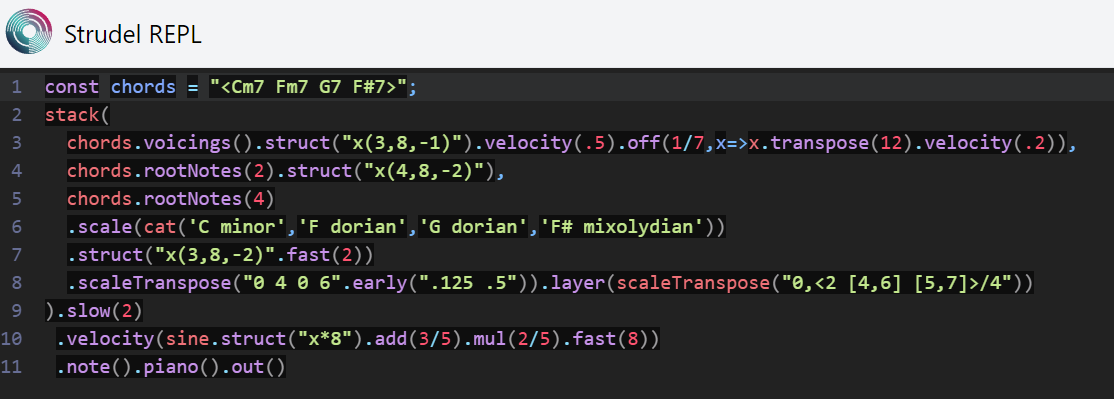
\includegraphics[scale=0.5]{images/strudel.png}
    \caption{The Strudel REPL (web-based application which runs Strudel), with example code/music}
    \label{fig:strudel}
\end{figure}

Another example of a live coding platform that I could work with is Sonic Pi, which is a standalone application with a much simpler language to write music and more in-depth tools than Strudel, but it is more limiting in the ease of expressiveness of the language. It is written in C++ and Ruby. It also uses SuperCollider to generate audio.
\section*{Starting Point}
I have very little experience with live coding and digital audio generation. I have no experience working in JavaScript or Ruby. I will need to learn about how Strudel and Sonic Pi work during the project, and will need to learn how to work with JavaScript or Ruby.
\section*{Substance of Project}
\subsection*{Core}
I will produce a piece of software which allows users to write code and generate audio from speech sounds in order to create music. Users will be able to take small snippets of speech and combine them by playing them back in a chosen order, with a chosen rhythm, by layering them, and by manipulating them in various ways.

I will also produce a piece of software which allows user to achieve a similar goal through diagrammatic means. A GUI will allow a user to take small speech literals as blocks and order them, pass them through filters, layer them or loop them.

Although tools exist that already allow you to do what my project will achieve, it will greatly improve the efficiency for a style of composition which, to my knowledge, has no tools dedicated to enabling it. You can achieve what my project will achieve in a standard DAW, but my tool will allow users to achieve more complicated rhythms and structures in much less time than they would moving samples of speech around in a DAW. It also makes the process much more accessible, allowing users with little experience working with digital composition tools or with programming to work with this style of proposition and to work with live coding techniques.
\subsection*{Extensions}
Some possibles extensions of my project would:
\begin{itemize}
    \item Build an explicit formal language describing the composition and generation of audio, based on the text-based tool.
    \item Change the text-based tool to reflect the definition of the formal language.
    \item Change the graphical tool to represent this formal language.
    \item Integrate neural synthesis of speech sounds into my composition tool. Antoine Caillon and Philippe Esling released a paper last year detailing a variational auto-encoder they have developed (RAVE) which allows for fast, high quality audio synthesis. I could implement RAVE into the tool to allow users to generate their own speech audio with state-of-the-art neural synthesis, adjusting parameters to change the sound in real time.
\end{itemize}
\section*{Success Criterion}
In order to have succeeded in my project, I require:
\begin{itemize}
    \item Software which allows users to write code which will use speech sounds to generate an audio output.
    \item Software which allows users to rearrange blocks specifying speech sounds and operations on those sounds in order to generate an audio output.
    \item Both pieces of software should allow for users to:
    \begin{itemize}
        \item Play back a small sample of speech.
        \item Arrange multiple sounds to be played back with a particular rhythm and order.
        \item Layer multiple sounds to be played alongside each other.
        \item Manipulate sounds with filters and effects.
    \end{itemize}
    \item The software be evaluated against an industry-standard DAW in user tests to express the efficacy of both the graphical and text-based tool in the production of phonological music.
\end{itemize}
For the final bullet point, I will supply the software to users who will give written feedback on the ease of use of my tool and existing tools. I will also measure the time taken for users to complete specific tasks to measure quantitatively the improvement on certain tasks over existing tools. I will use A/B testing to compare the two implementations, text-based and graphical, to measure the ease of use for each tool.
\section*{Timetable}
\subsection*{Feedback}
Over the duration of my project, I plan to interact with users for feedback. I am already in contact with one artist and I will venture to find other possible users of my tool through people I know and get feedback from a wider source. In the first few weeks, I will need to fill in the form for the Ethics Committee to approve the involvement of human participants.
\subsection*{Week 1/2: 16th Oct. - 29th Oct.}
\begin{itemize}
    \item Study Strudel framework.
    \item Study Sonic Pi framework.
    \item Set up work environment for development of text-based tool.
\end{itemize}
{
\centering\textbf{Milestone:} Decide whether to work with Strudel or Sonic Pi, supplying a report describing the details of the research and my choice to my supervisor. Be able to compile and run Strudel and/or Sonic Pi on my own machine, allowing for my own modifications and additions to the code.
}
\subsection*{Week 3/4: 30th Oct. - 12th Nov.}
\begin{itemize}
    \item Research system for generation of audio.
    \item Understand how to generate, combine and manipulate audio to produce new outputs.
\end{itemize}
{
\centering\textbf{Milestone:} Write program which is able to generate sample audio outputs, working on samples given by user.
}
\subsection*{Week 5/6: 13th Nov. - 26th Nov.}
\begin{itemize}
    \item Begin programming of text-based composition tool.
\end{itemize}
{
\centering\textbf{Milestone:} Have functioning text-based tool which allows users to input code and generate audio using small snippets of speech.
}
\subsection*{Week 7/8: 27th Nov. - 10th Dec.}
\textit{Michaelmas term ends: 1st Dec. Varsity skiing trip}
\begin{itemize}
    \item Continue work on text-based tool.
    \item Test text-based implementation on user, get feedback.
\end{itemize}
{
\centering\textbf{Milestone:} Report describing user feedback, possible improvements and tweaks to system.
}
\subsection*{Week 9/10: 11th Dec. - 24th Dec.}
\begin{itemize}
    \item Refine text-based tool based on feedback.
\end{itemize}
{
\centering\textbf{Milestone:} New, improved version of tool modified based on the feedback from the user.
}
\subsection*{Week 11/12: 25th Dec. - 7th Jan.}
\textit{Christmas and New Years Eve, will not be completing much work.}
\begin{itemize}
    \item Research libraries for creating visual programming languages (e.g. Blockly).
\end{itemize}
{
\centering\textbf{Milestone:} Write up a page for project supervisor describing what I have learnt, what library I will use and how I will use the library to create a GUI.
}
\subsection*{Week 13/14: 8th Jan. - 21st Jan.}
\textit{Lent term starts: 17th Jan.}
\begin{itemize}
    \item Build diagrammatic tool for phonological audio composition.
\end{itemize}
{
\centering\textbf{Milestone:} Working GUI, allowing users to rearrange blocks in order to generate audio in different ways.
}
\subsection*{Week 15/16: 22nd Jan. - 4th Feb.}
\textit{Progress deadline due: 3rd Feb (12pm)}
\begin{itemize}
    \item Feedback from user.
    \item Improve on GUI.
    \item Write progress report.
\end{itemize}
{
\centering\textbf{Milestone:} Hand-in progress report, written evaluation of user feedback.
}
\subsection*{Week 17/18: 5th Feb. - 18th Feb.}
\begin{itemize}
    \item Start writing the dissertation.
\end{itemize}
{
\centering\textbf{Milestone:} Complete draft chapter to be reviewed by project supervisor.
}
\subsection*{Week 19/20: 19th Feb. - 4th Mar.}
\textit{Slack: time for me to catch up if running behind, complete extensions if ahead.}
\subsection*{Week 21/22: 5th Mar. - 18th Mar.}
Continue to write dissertation.

{
\centering\textbf{Milestone:} Draft of Introduction, Preparation chapters to be sent to supervisor.
}
\subsection*{Week 23/24: 19th Mar. - 1st Apr.}
Continue to write dissertation.
{

\centering\textbf{Milestone:} Draft of Implementation, Evaluation chapters to be sent to supervisor.
}
\subsection*{Week 25/26: 2nd Apr. - 15th Apr.}
Continue to write dissertation.

{
\centering\textbf{Milestone:} Full draft of dissertation to be sent to supervisor.
}
\subsection*{Week 27/28: 16th Apr. - 29th Apr.}
\textit{Slack: time for me to push back goals into.}
\subsection*{Week 29/30: 30th Apr. - 12th May}
\begin{itemize}
    \item Final touch-ups.
    \item Hand in final dissertation.
\end{itemize}
{
\centering\textbf{Milestone:} Finish project!
}

\textit{Note: During the weeks of writing the dissertation, I will periodically be sending the drafts to my supervisor for feedback, and improving on them when feedback is received.}
\section*{Resource Declaration}
My own laptop is sufficient to complete this project. No particularly heavy computation will be necessary. I don't have much storage left on my laptop, so I will need to acquire an extra SSD. The software and libraries that I will be using in this project is all publicly available (Strudel, Blockly, Sonic Pi, SuperDirt,  etc.). I will use a GitHub repository to store my code as well as my own laptop storage, and so in case of a failure of my laptop I will have a back-up of my work.
\textit{I accept full responsibility for this machine and I have made contingency plans to protect myself against hardware and/or software failure.}
\end{document}


\end{document}